\chapter{Ошибки и процессы}
\label{errors-and-processes}
\section{Связи}
\label{links}
Связи \--- это особый вид взаимоотношений, которые могут быть установлены между двумя процессами.
Когда один из процессов, который участвует в таких отношениях, умирает от неожиданного броска, ошибки или завершения (см. \ref{errors-and-exceptions} Ошибки и исключения), то связанный с ним процесс тоже завершается.

Эта концепция может пригодиться, когда требуется как можно быстрее завершить процесс, чтобы предотвратить появление ошибок.
Если процесс, в котором появилась ошибка, завершился аварией, а процессы, которые на него полагаются, продолжили работать, то все эти зависимые процессы должны что\--то предпринять.
Обычно приемлемым вариантом развития событий можно считать остановку и перезапуск всей группы процессов.
Именно это и позволяют нам сделать связи.

Для создания связи между двумя процессами в Erlang существует базовая функция \href{http://erldocs.com/R15B/erts/erlang.html\#link/1}{link/1}, принимающая в качестве аргумента Pid.
После запуска эта функция создаст связь между текущим процессом и процессом, который отождествляется с указанным \emph{Pid}.
Для разрушения связи используют функцию \href{http://erldocs.com/R15B/erts/erlang.html\#unlink/1}{unlink/1}.
При аварийном завершении одного из связанных процессов, отсылается сообщение особого вида, которое несёт информацию относительно произошедших событий.
Если процесс умирает по естественным причинам (читай: завершает исполнение своих функций), то такое сообщение не отсылается.
Для начала поговорим об этой новой функции как об элементе модуля \href{http://learnyousomeerlang.com/static/erlang/linkmon.erl}{linkmon.erl}:
\begin{lstlisting}[style=erlang]
myproc() ->
    timer:sleep(5000),
    exit(reason).
\end{lstlisting}

Если вы попробуете исполнить следущие вызовы функций (и сделаете между каждой командой spawn пятисекундную паузу), то увидите, что оболочка завершится с ошибкой 'reason' только если между двумя процессами была установлена связь.
\begin{lstlisting}[style=erlang]
1> c(linkmon).
{ok,linkmon}
2> spawn(fun linkmon:myproc/0).
<0.52.0>
3> link(spawn(fun linkmon:myproc/0)).
true
** exception error: reason
\end{lstlisting}

Изобразим это на картинке:
\begin{figure}[h!]
    \centering
    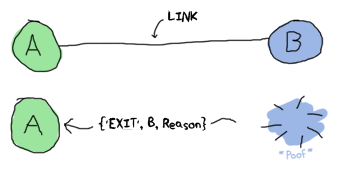
\includegraphics[width=0.7\textwidth]{link-exit.png}
\end{figure}

Для захвата сообщения \ops{\{'EXIT', B, Reason\}} не получится использовать стандартную структуру \ops{try \ldots catch}.
Для этого существуют другие средства, которые мы рассмотрим позже.

Важно отметить, что связи можно также использовать, для организации больших групп процессов, которые должны прекращать исполнения как единая группа, все вместе:
\begin{lstlisting}[style=erlang]
chain(0) ->
    receive
        _ -> ok
    after 2000 ->
        exit("chain dies here")
    end;
chain(N) ->
    Pid = spawn(fun() -> chain(N-1) end),
    link(Pid),
    receive
        _ -> ok
    end.
\end{lstlisting}

Эта функция принимает целое число \emph{N}, запускает \emph{N} связанных между собой процессов.
Для передачи \emph{N-1} аргумента следующему процессу в <<цепи>>, я оборачиваю вызов в анонимную функцию, чтобы она перестала принимать аргументы.
Подобный эффект можно получить при помощи вызова \ops{spawn(?MODULE, chain, [N-1])}.

В этом примере я создам множество связанных процессов, которые будут умирать сразу после завершения их наследников:
\begin{lstlisting}[style=erlang]
4> c(linkmon).              
{ok,linkmon}
5> link(spawn(linkmon, chain, [3])).
true
** exception error: "chain dies here"
\end{lstlisting}

Как видите, оболочка получает сообщение о смерти от одного из процессов.
Вот подробное описание завершения запущенных процессов и уничтожения связей:
\begin{lstlisting}[style=erlang]
[shell] == [3] == [2] == [1] == [0]
[shell] == [3] == [2] == [1] == *dead*
[shell] == [3] == [2] == *dead*
[shell] == [3] == *dead*
[shell] == *dead*
*dead, error message shown*
[shell] <-- restarted
\end{lstlisting}

После завершения процесса, который исполняет функцию \ops{linkmon:chain(0)}, ошибка передаётся по цепи связей, и в результате из\--за неё умирает процесс оболочки.
Авария могла произойти в любом из связанных процессов.
Связи работают в обе стороны, поэтому для завершения всей группы процессов достаточно смерти лишь одного из них.\\
\colorbox{lgray}
{
\begin{minipage}{1.0\linewidth}
    \textbf{Замечание:} если вам необходимо убить из оболочки какой\--либо процесс, то это можно сделать при помощи функции \href{http://erldocs.com/R15B/erts/erlang.html\#exit/2}{exit/2}.
    Её можно вызвать следующим образом: \ops{exit(Pid, Reason)}.
    Можете попробовать ею воспользоваться, если хотите.
\end{minipage}
}
\colorbox{lgray}
{
\begin{minipage}{1.0\linewidth}
    \textbf{Замечание:} связи не накапливаются.
    Если вы вызвали \ops{link/1} 15 раз для одной и той же пары процессов, то между ними будет существовать лишь одна связь, и для её разрушения будет достаточно однократного вызова \ops{unlink/1}.
\end{minipage}
}

Нужно сказать, что вызовы \ops{link(spawn(Function))} или \ops{link(spawn(M,F,A))} совершаются в несколько шагов.
Иногда процесс может умереть до того как была установлена связь, и это спровоцирует неожиданное поведение исполняемого кода.
На такой случай в языке существует функция \href{http://erldocs.com/R15B/erts/erlang.html\#spawn_link/1}{spawn\_link/1-3}.
Она принимает те же самые параметры, что и \ops{spawn/1-3}, создаёт процесс и связывает его, так же как это делает \ops{link/1}, но весь процесс осуществляется атомарной операцией (все действия объединяются в одно, и результатом их исполнения может стать лишь совокупный успех или неудача, никаких других результатов быть не может).
Такой способ создания процессов и их связей считается более надёжным.
К тому же, на нём можно сэкономить пару скобок.
\section{Это ловушка!}
\label{its-a-trap}
\begin{wrapfigure}{r}{0.35\linewidth}
    
\includegraphics[width=1\linewidth]{ackbar.jpg}
\end{wrapfigure}
Вернёмся к связям и умирающим процессам.
Распространение ошибок от процесса к процессу осуществляется методом, похожим на передачу сообщений, но при этом используется их особый тип \--- сигналы.
Сигналы о завершении \--- это <<тайные>> сообщения, которые автоматически действуют на процессы, убивая их во время исполнения.

Я уже неоднократно упоминал, что надёжность приложения зависит от его умения быстро убивать и перезапускать процессы.
На текущий момент в качестве орудия убийства можно использовать связи.
Осталось разобраться с перезапуском.

Чтобы перезапустить процесс, сначала нужно как\--то узнать, что он умер.
Мы можем сделать это, добавив поверх связей ещё один слой (вкусную глазурь на торте), содержащий концепцию, которая называется \emph{системные процессы} (system processes).
Системные процессы, по сути, это обычные процессы, но они могут конвертировать сигналы о завершении в обычные сообщения.
Делают они это при помощи вызова \ops{process\_flag(trap\_exit, true)} в работающем процессе.
Ничто не сможет рассказать об этом механизме больше, чем пример.
Поэтому сейчас мы его и рассмотрим.
Я немного видоизменю пример с chain, поместив в начале системный процесс:
\begin{lstlisting}[style=erlang]
1> process_flag(trap_exit, true).
true
2> spawn_link(fun() -> linkmon:chain(3) end).
<0.49.0>
3> receive X -> X end.
{'EXIT',<0.49.0>,"chain dies here"}
\end{lstlisting}

Ага!
Это уже интереснее.
Вернёмся к нашей иллюстрации.
Теперь картина событий выглядит приблизительно так:
\begin{lstlisting}[style=erlang]
[shell] == [3] == [2] == [1] == [0]
[shell] == [3] == [2] == [1] == *dead*
[shell] == [3] == [2] == *dead*
[shell] == [3] == *dead*
[shell] <-- {'EXIT,Pid,"chain dies here"} -- *dead*
[shell] <-- still alive!
\end{lstlisting}

Вот он, механизм позволяющий быстро перезапускать процессы.
Используя системные процессы при написании программ, можно легко создать процесс, единственная функция которого \--- следить за тем, чтобы все процессы оставались живы, и рестартовать их в случае аварии.
Мы поговорим об этом подробнее в следующей главе, когда будем применять этот приём по\--настоящему.

А сейчас я хочу вернуться к функциям для работы с исключениями, которые мы рассмотрели в главе ~\ref{errors-and-exceptions} об ошибках и исключениях, и увидим как они ведут себя в процессах, которые улавливают факт завершения других процессов.
Сначала  определим основание для эксперимента, не используя системный процесс.
Я последовательно приведу результаты, которые возвращают непойманные броски, ошибки и завершения (exits) в соседних процессах:

\begin{itemize}
    \item \textbf{Источник исключения:} \ops{spawn\_link(fun() -> ok end)}\\
    \textbf{Результат, который не был словлен:} - nothing -\\
    \textbf{Словленный результат:} \{'EXIT', <0.61.0>, normal\}\\
    Процесс завершился в обычном порядке, без проблем.
    Заметьте, что этот результат выглядит почти так же как и результат \ops{catch\_exit(normal)}, с тем лишь отличием, что для идентификации проблемного процесса в кортеж добавлен PID.\\
    \item \textbf{Источник исключения:} \ops{spawn\_link(fun() -> exit(reason) end)}
    \textbf{Результат, который не был словлен:} ** exception exit: reason\\
    \textbf{Словленный результат:} \{'EXIT', <0.55.0>, reason\}\\
    Процесс завершился по причине, указанной пользователем.\\
    В данном случае, если не было словлено завершение (exit), то процесс аварийно прекращает работу.\\
    В противном случае вы получите сообщение, указанное выше.\\
    \item \textbf{Источник исключения:} \ops{spawn\_link(fun() -> exit(normal)  end)}
    \textbf{Результат, который не был словлен:} - nothing -\\
    \textbf{Словленный результат:} \{'EXIT', <0.58.0>, normal\}\\
    Этот вызов эмулирует нормальное завершение процесса.
    Иногда в ходе обычного  исполнения программы нужно убить процесс, не создавая никаких исключений.
    В этом  случае применяют именно такой метод.\\
    \item \textbf{Источник исключения:} \ops{spawn\_link(fun() -> 1/0 end)}
    \textbf{Результат, который не был словлен:} Error in process <0.44.0> with exit value: \{badarith, [\{erlang, '/', [1,0]\}]\}\\
    \textbf{Словленный результат:} \{'EXIT', <0.52.0>, \{badarith, [\{erlang, '/', [1,0]\}]\}\}\\
    Ошибка (\ops{\{badarith, Reason\}}) не перехватывается блоком \ops{try \ldots catch} и передаётся выше, достигая 'EXIT'.
    С этого момента вызов ведёт себя так же как и \ops{exit(reason)}, c той разницей, что трассировка стека будет содержать более полную информацию о произошедшем.\\
    \item \textbf{Источник исключения:} \ops{spawn\_link(fun() -> erlang:error(reason) end)}
    \textbf{Результат, который не был словлен:} Error in process <0.47.0> with exit value: \{reason, [\{erlang, apply, 2\}]\}\\
    \textbf{Словленный результат:} \{'EXIT', <0.74.0>, \{reason, [\{erlang, apply, 2\}]\}\}\\
    Этот вызов почти такой же как \ops{1/0}.
    Ничего особенного в этом нет, так как \ops{erlang:error/1} создан для использования именно в такой ситуации.\\
    \item \textbf{Источник исключения:} \ops{spawn\_link(fun() -> throw(rocks) end)}
    \textbf{Результат, который не был словлен:} Error in process <0.51.0> with exit value: \{\{nocatch, rocks\}, [\{erlang, apply, 2\}]\}\\
    \textbf{Словленный результат:} \{'EXIT', <0.79.0>, \{\{nocatch, rocks\}, [\{erlang, apply, 2\}]\}\}\\
    Бросок (throw) не перехватывается блоком \ops{try\ldots catch}  и переходит в ошибку (error), которая переходит в EXIT.
    Если процесс не ловит exit, его исполнение заканчивается аварией.
    В противном случае всё проходит без каких\--либо проблем.
\end{itemize}

Вот, пожалуй, и всё, что я хотел рассказать об обычных исключениях.
Если дела идут как обычно \--- всё проходит нормально.
Случается что\--то исключительное \--- умирает процесс, рассылаются различные сигналы.

А ещё есть \ops{exit/2}.
Этот вызов \--- что\--то вроде пистолета, который могут использовать процессы в Erlang.
Он позволяет процессу убить другой процесс, сохраняя безопасную дистанцию.
Вот некоторые вызовы, которые можно делать с его помощью:
\begin{itemize}
    \item 
        \textbf{Источник исключения:} \ops{exit(self(), normal)}\\
    \textbf{Результат, который не был словлен:} ** exception exit: normal\\
    \textbf{Словленный результат:} \{'EXIT', <0.31.0>, normal\}\\
    Когда вызов \ops{exit(self(), normal)} не улавливает завершения (exits), он действует так же как и \ops{exit(normal)}.
    В противном случае, вы получаете сообщение того же формата, который можно получить при прослушивании связей (links) от умирающих внешних (foreign) процессов.
\item 
    \textbf{Источник исключения:} \ops{exit(spaen\_link(fun() -> timer:sleep(50000) end), normal)}\\
    \textbf{Результат, который не был словлен:} - nothing -\\
    \textbf{Словленный результат:} - nothing -\\
    Фактически, это вызов функции \ops{exit(Pid, normal)}.
    Ничего полезного эта команда не делает, так как процесс нельзя удалённо убить с причиной \ops{normal} в качестве аргумента.
\item
    \textbf{Источник исключения:} \ops{exit(spawn\_link(fun() -> timer:sleep(50000) end), reason)}\\
    \textbf{Результат, который не был словлен:} ** exception exit: reason\\
    \textbf{Словленный результат:} \{'EXIT', <0.52.0>, reason\}\\
    Внешний (foreign) процесс завершает себя по причине \emph{reason}.
    Выглядит это так, как будто внешний процесс сам для себя сделал вызов \ops{exit(reason)}.
\item
    \textbf{Источник исключения:} \ops{exit(spawn\_link(fun() -> timer:sleep(50000) end), kill)}\\
    \textbf{Результат, который не был словлен:} ** exception exit: killed\\
    \textbf{Словленный результат:} \{'EXIT', <0.58.0>, killed\}\\
    Удивительно, но на пути от умирающего процесса к источнику, сообщение изменяется.
    Теперь создатель процесса получает \ops{killed} вместо {kill}.
    Происходит это потому, что \ops{kill} \--- особенный сигнал завершения.
    Подробнее об этом чуть позже.
\item
    \textbf{Источник исключения:} \ops{exit(self(), kill)}\\
    \textbf{Результат, который не был словлен:} ** exception exit: killed\\
    \textbf{Словленный результат:} ** exception exit: killed\\
    Ого, глядите\--ка.
    Похоже, это исключение словить невозможно.
    Ну\--ка проверим.
\item
    \textbf{Источник исключения:} \ops{spawn\_link(fun() -> exit(kill) end)}\\
    \textbf{Результат, который не был словлен:} ** exception exit: killed\\
    \textbf{Словленный результат:} \{'EXIT', <0.67.0>, kill\}\\
    Немного запутанно.
    Когда какой\--либо процесс убивает себя вызовом \ops{exit(kill)}, и мы не улавливаем завершения (exits), то наш собственный процесс умирает с причиной \ops{killed}.
    Но если мы ловим завершения, этого не происходит.
\end{itemize}

Хотя большинство причин завершения поддаются улавливанию, всё же есть ситуации, в которых вам понадобилось бы жестоко расправиться с неким процессом.
Такой процесс, к примеру,  ловит завершения (exits), но застрял в бесконечном цикле и игнорирует все сообщения.
Причина завершения \ops{kill} действует как особый сигнал, который невозможно уловить.
Таким образом мы гарантируем, что любой процесс, завершаемый по этой причине, действительно будет мёртв.
К \ops{kill} обычно прибегают как к крайней мере, когда больше ничего не срабатывает.
\begin{wrapfigure}{r}{0.4\linewidth}
    
\includegraphics[width=1\linewidth]{trap.png}
\end{wrapfigure}

Так как причину завершения \ops{kill} словить невозможно, её необходимо заменять на \ops{killed} до того как другой процесс получит это сообщение. 
Если такую замену не сделать, то каждый процесс, связанный с умирающим, умрёт от той же самой причины \ops{kill}, и, в свою очередь, убьёт своих соседей, и так далее.
Смерть будет распространяться каскадами.

Этот факт также объясняет, почему \ops{exit(kill)} выглядит так же как и \ops{killed} при его получении другими связанными процессами (перед получением сигнал видоизменяется, и цепной реакции не происходит), но будучи захвачен локально, он выглядит как \ops{kill}.

Если вас всё это запутало, не переживайте.
Множество программистов испытывают те же чувства.
Сигналы завершения \-- странные твари.
К счастью, кроме описанных выше ситуаций, существует не так уж много вариантов их использования.
После усвоения этих примеров, вам будет ясна большая часть механизмов конкурентного управления ошибками в Erlang.
\section{Мониторы}
\label{monitors}
Ну, ладно.
Может, вам совсем не хочется жестоко убивать процессы.
Может, вы не собираетесь разрушить весь мир и погибнуть вместе с ним.
Может, вам больше нравится наблюдать.
Тогда мониторы придутся вам по вкусу.

Если серьёзно, то мониторы представляют собой особый тип связей с двумя отличиями:
\begin{itemize}
    \item они работают в одну сторону;
    \item их можно накапливать (stack).
\end{itemize}

\begin{wrapfigure}{l}{0.21\linewidth}
    
\includegraphics[width=1\linewidth]{homer.png}
\end{wrapfigure}

Мониторы могут пригодиться, когда какой\--либо процесс хочет знать, что происходит с другим  процессом, но это знание не представляет жизненной ценности ни для кого из них.

Ещё одна причина, которая приведена в списке \--- это возможность накопления (stacking) ссылок.
На первый взгляд она может показаться бесполезной, но эта характеристика очень полезна при написании библиотек, для функционирования которых необходимо знать, что происходит с другими процессами.

Нужно понимать, что связи в большей степени относятся к средствам организации.
При проектировании архитектуры вашего приложения, различным процессам назначаются их функции, и между ними строятся зависимости.
Некоторые процессы будут присматривать за другими, кто\--то из них не сможет существовать без парного процесса и т.д.
Обычно эта структура существует как нечто предрешённое, известное наперёд.
Именно в такую ситуацию органично вписываются связи, и использовать их в другом окружении совсем не обязательно.

Но что делать, если вы пользуетесь 2\--мя или 3\--мя разными библиотеками, и всем им необходимо знать, жив процесс или нет?
Если бы вы для этого использовали связи, то очень скоро столкнулись бы с проблемой при отвязке процесса.
Нужно понимать, что связи нельзя накапливать, поэтому как только вы разрушите одну связь, больше связей не останется, и все предположения об их существовании, которые делают различные библиотеки, будут нарушены.
Хорошего мало.
Поэтому вам понадобятся связи, которые можно накапливать, наслаивать поверх друг друга, и мониторы эту проблему решают.
Их можно удалять по отдельности.
К тому же, их однонаправленность удобно использовать в библиотеках, так как другим процессам о существовании этих библиотек знать совершенно не нужно.

Так как же выглядит монитор?
Давайте просто создадим его и посмотрим.
Для этого используют функцию \href{http://erldocs.com/R15B/erts/erlang.html\#monitor/2}{erlang:monitor/2}, первым параметром которой является атом \emph{process}, а вторым \--- pid процесса:
\begin{lstlisting}[style=erlang]
1> erlang:monitor(process, spawn(fun() -> timer:sleep(500) end)).
#Ref<0.0.0.77>
2> flush().
Shell got {'DOWN',#Ref<0.0.0.77>,process,<0.63.0>,normal}
ok
\end{lstlisting}

Каждый раз, когда наблюдаемый процесс прекращает работать, вы получаете сообщение вида \ops{\{'DOWN', MonitorReference, process, Pid, Reason\}}.
Ссылка позволяет прекратить наблюдение за процессом.
Помните, что мониторы можно накапливать, так что при желании можно не ограничиваться выключением только одного монитора.
Ссылки позволяют следить за каждым по отдельности.
Как и для ссылок, для мониторов существует атомарная функция, которая позволяет создать процесс и сразу начать за ним наблюдение \--- \href{http://erldocs.com/R15B/erts/erlang.html\#spawn_monitor/1}{spawn\_monitor/1-3}:
\begin{lstlisting}[style=erlang]

3> {Pid, Ref} = spawn_monitor(fun() -> receive _ -> exit(boom) end end).
{<0.73.0>,#Ref<0.0.0.100>}
4> erlang:demonitor(Ref).
true
5> Pid ! die.
die
6> flush().
ok
\end{lstlisting}

В этом примере мы прекращаем наблюдать за процессом до его завершения, и поэтому не видим как он умирает.
Существует также функция \href{http://erldocs.com/R15B/erts/erlang.html\#demonitor/2}{demonitor/2}, которая позволяет извлечь чуть больше информации.
Вторым параметром ей можно передавать список опций.
Их всего лишь две: \ops{info} и \ops{flush}:
\begin{lstlisting}[style=erlang]
7> f().
ok
8> {Pid, Ref} = spawn_monitor(fun() -> receive _ -> exit(boom) end end).
{<0.35.0>,#Ref<0.0.0.35>}
9> Pid ! die.
die
10> erlang:demonitor(Ref, [flush, info]).
false
11> flush().
ok
\end{lstlisting}

Опция \ops{info} сообщает о том, существовал ли монитор в момент попытки его удаления.
Именно поэтому выражение 10 вернуло \ops{false}.
При помощи \ops{flush} можно удалить сообщение \ops{DOWN} из почтового ящика, если оно там, конечно, было.
После этого функция \ops{flush()} ничего в ящике текущего процесса не найдёт.
\section{Присваиваем процессам имена}
Мы разобрались со связями и мониторами, осталось решить ещё одну проблему.
Давайте воспользуемся следующей функцией из модуля \href{http://learnyousomeerlang/original/learnyousomeerlang.com/static/erlang/linkmon.erl}{linkmon.erl}:
\begin{lstlisting}[style=erlang]
start_critic() ->
spawn(?MODULE, critic, []).
 
judge(Pid, Band, Album) ->
    Pid ! {self(), {Band, Album}},
    receive
        {Pid, Criticism} -> Criticism
    after 2000 ->
        timeout
    end.
 
critic() ->
    receive
        {From, {"Rage Against the Turing Machine", "Unit Testify"}} ->
            From ! {self(), "They are great!"};
        {From, {"System of a Downtime", "Memoize"}} ->
            From ! {self(), "They're not Johnny Crash but they're good."};
        {From, {"Johnny Crash", "The Token Ring of Fire"}} ->
            From ! {self(), "Simply incredible."};
        {From, {_Band, _Album}} ->
            From ! {self(), "They are terrible!"}
    end,
    critic().
\end{lstlisting}

А теперь мы просто представим, что ходим по магазинам, покупаем музыкальные записи.
Некоторые альбомы звучат неплохо, но полной уверенности на их счёт у вас нет.
Вы решаете позвонить другу \--- музыкальному критику.
\begin{lstlisting}[style=erlang]
1> c(linkmon).                        
{ok,linkmon}
2> Critic = linkmon:start_critic().
<0.47.0>
3> linkmon:judge(Critic, "Genesis", "The Lambda Lies Down on Broadway").
"They are terrible!"
\end{lstlisting}

Из\--за солнечной бури (я стараюсь придумать что\--то правдоподобное), соединение разрывается:
\begin{lstlisting}[style=erlang]
4> exit(Critic, solar_storm).
true
5> linkmon:judge(Critic, "Genesis", "A trick of the Tail Recursion").
timeout
\end{lstlisting}

Вот досада.
Больше критику о наших альбомах мы получать не можем.
Чтобы критик оставался на связи, мы напишем простой процесс <<супервизор>> (supervisor), единственной задачей которого будет перезапуск критика, если тот прекращает исполнение:
\begin{lstlisting}[style=erlang]
start_critic2() ->
    spawn(?MODULE, restarter, []).
 
restarter() ->
    process_flag(trap_exit, true),
    Pid = spawn_link(?MODULE, critic, []),
    receive
        {'EXIT', Pid, normal} -> % not a crash
            ok;
        {'EXIT', Pid, shutdown} -> % manual termination, not a crash
            ok;
        {'EXIT', Pid, _} ->
            restarter()
    end.
\end{lstlisting}

Ответственный за перезапуск будет сам представлен в виде процесса.
В свою очередь, он запустит процесс\--критик, и если тот когда\--либо умрёт по причине аварии, \ops{restarter/0} пройдёт одну итерацию цикла и создаст нового критика.
Обратите внимание, что шаблон \ops{\{'EXIT', Pid, shutdown\}} я добавил как средство для ручного останова критика, на случай если нам когда\--либо захочется это сделать.

В нашем подходе к решению этой проблемы есть один изъян: мы не можем узнать Pid критика, а поэтому мы не можем ему позвонить, чтобы осведомиться о его мнении.
Одним из решений этой проблемы в Erlang является именование процессов.

Присвоение имени процессу позволяет вам заменять непредсказуемый pid на атом.
Затем этот атом можно использовать при отсылке сообщений совершенно так же как Pid.
Для именования процесса используется функция \href{http://erldocs.com/R15B/erts/erlang.html\#register/2}{erlang:register/2}.
Если процесс умирает, он автоматически теряет имя.
Для удаления имени вручную можно использовать \href{http://erldocs.com/R15B/erts/erlang.html\#unregister/1}{unregister/1}.
Получить список зарегистрированных процессов можно при помощи \href{http://erldocs.com/R15B/erts/erlang.html\#registered/0}{registered/0}, а более подробный список возвращает команда оболочки \ops{regs()}.
Давайте придадим функции \ops{restarter/0} следующий вид:
\begin{lstlisting}[style=erlang]
restarter() ->
    process_flag(trap_exit, true),
    Pid = spawn_link(?MODULE, critic, []),
    register(critic, Pid),
    receive
        {'EXIT', Pid, normal} -> % not a crash
            ok;
        {'EXIT', Pid, shutdown} -> % manual termination, not a crash
            ok;
        {'EXIT', Pid, _} ->
            restarter()
    end.
\end{lstlisting}

Как видите, независимо от Pid критика, функция \ops{register/2} всегда будет давать ему имя <<critic>>.
Теперь нам нужно убрать необходимость передачи Pid из функции абстракции.
Попробуем сделать это так:
\begin{lstlisting}[style=erlang]
judge2(Band, Album) ->
    critic ! {self(), {Band, Album}},
    Pid = whereis(critic),
    receive
        {Pid, Criticism} -> Criticism
    after 2000 ->
        timeout
    end.
\end{lstlisting}

В этом примере строка \ops{Pid = whereis(critic)} используется для определения идентификатора процесса\--критика, для того чтобы подставить его в сопоставление с образцом в выражении \ops{receive}.
Нам необходимо это сопоставление, так как оно позволяет убедиться, что мы будем обрабатывать правильное сообщение (на этот момент в почтовом ящике может быть, скажем, 500 сообщений!)
Но этот подход может стать источником проблем.
Вышеприведённый код предполагает, что pid критика не будет изменяться между первыми двумя строками функции.
Но вполне можно предположить, что случится следующее:
\begin{verbatim}
  1. critic ! Message
                        2. critic получает сообщение
                        3. critic отвечает
                        4. critic умирает
  5. в функции whereis происходит сбой
                        6. critic перезапускается
  7. происходит аварийное завершение кода
\end{verbatim}

Нельзя исключать и такой вариант:
\begin{verbatim}
  1. critic ! Message
                           2. critic получает сообщение
                           3. critic отвечает
                           4. critic умирает
                           5. critic перезапускается
  6. функция whereis получает неверный pid
  7. сообщение никогда не пройдёт сопоставление с образцом
\end{verbatim}

Существует вероятность, что если мы не сделаем всё как следует, то ошибка в одном процессе вызовет ошибку в другом.
В этом случае значение атома \emph{critic} будет доступно  сразу в нескольких процессах.
Это называется \emph{разделяемым состоянием}.
Проблема заключается в том, что значение \emph{critic} может считываться \emph{и} изменяться разными процессами практически в один и тот же момент.
Это приводит данные к противоречивому виду и может вызвать ошибки в программном обеспечении.
Такое состояние обычно называют <<состоянием гонки>> \emph{race condition}.
Они очень опасны тем, что зависят от распределения событий во времени.
Практически в любом конкурентном и параллельном языке это распределение зависит от непредсказуемых факторов, таких, например, как загрузка процессора, распределение процессов и того, какие данные обрабатываются вашей программой.\\
\colorbox{lorange}
{
\begin{minipage}{1.0\linewidth}
    \textbf{Не забывайтесь:} 
Возможно, вы слышали, что обычно в Erlang нет <<состояний гонки>> (race conditions) или взаимных блокировок (deadlocks), что, в свою очередь, обеспечивает надёжность параллельного кода.
Во многих случаях это действительно так, но никогда не полагайтесь на то, что ваш код действительно абсолютно надёжен.
Помимо именованных процессов существует ещё много способов заставить параллельный код исполняться не так как было задумано.\\
\\
Как пример можно привести доступ к файлам, размещённым на диске компьютера (с целью их модификации), обновление одних и тех же записей в базе данных сразу из нескольких процессов и т.д.
\end{minipage}
}

К счастью, код, приведённый выше, сравнительно легко можно исправить.
Необходимо лишь предположить, что именованный процесс не всегда будет оставаться тем же, и для идентификации сообщений использовать ссылки (которые можно создавать при помощи \ops{make\_ref()}.
Нам понадобится заменить функцию \ops{critic/0} на \ops{critic2/0}, а \ops{judge/3} на \ops{judge2/2}:
\begin{lstlisting}[style=erlang]
judge2(Band, Album) ->
    Ref = make_ref(),
    critic ! {self(), Ref, {Band, Album}},
    receive
        {Ref, Criticism} -> Criticism
    after 2000 ->
        timeout
    end.
 
critic2() ->
    receive
        {From, Ref, {"Rage Against the Turing Machine", "Unit Testify"}} ->
            From ! {Ref, "They are great!"};
        {From, Ref, {"System of a Downtime", "Memoize"}} ->
            From ! {Ref, "They're not Johnny Crash but they're good."};
        {From, Ref, {"Johnny Crash", "The Token Ring of Fire"}} ->
            From ! {Ref, "Simply incredible."};
        {From, Ref, {_Band, _Album}} ->
            From ! {Ref, "They are terrible!"}
    end,
    critic2().
\end{lstlisting}

А затем поменять \ops{restarter/0} таким образом, чтобы он вместо \ops{critic/0} запускал \ops{critic2/0}.
Все остальные функции можно оставить без изменений.
Для пользователя эта модификация пройдёт незамеченной.
Точнее, он заметит, что мы переименовали функции и изменили несколько параметров, но он не узнает подробностей реализации, и почему эти изменения необходимо было сделать.
Он увидит только, что его код упростился, и что при вызове функций больше не нужно постоянно передавать pid:
\begin{lstlisting}[style=erlang]
6> c(linkmon).
{ok,linkmon}
7> linkmon:start_critic2().
<0.55.0>
8> linkmon:judge2("The Doors", "Light my Firewall").
"They are terrible!"
9> exit(whereis(critic), kill).
true
10> linkmon:judge2("Rage Against the Turing Machine", "Unit Testify").    
"They are great!"
\end{lstlisting}

Ну а теперь, даже если мы убили критика, мгновенно появляется новый, и решает наши проблемы.
Вот она, польза именованных процесов.
Если бы вы попытались вызвать \ops{linkmon:judge/2} без зарегистрированного процесса, то внутри функции оператором \ops{!} была бы выброшена ошибка \emph{bad argument}, которая гарантирует, что процессы, зависящие от именованного процесса, не смогут продолжить исполнение без него.\\
\colorbox{lgray}
{
\begin{minipage}{1.0\linewidth}
    \textbf{Замечание:} я уже упоминал, что атомы можно использовать для ограниченного круга ситуаций (хоть этот круг и достаточно велик).
Никогда не создавайте атомы динамически.
Это значит, что именованные процессы должны использоваться только для важных сервисов, уникальных в рамках одной VM, и эти процессы должны быть запущены на протяжении всего времени работы вашего приложения.\\
\\
Если вам понадобились именованные процессы, но их существование скоротечно, или их уникальность в рамках VM не может быть обеспечена, то скорее всего их нужно представить в виде группы.
По сравнению с использованием динамических имён, связывание и одновременный перезапуск группы процессов в случае аварии, может оказаться более разумным выбором.
\end{minipage}
}

В следующей главе мы применим свежеприобретённые знания о конкурентном программировании в Erlang для написания настоящих приложений.
